\documentclass{article}
\usepackage[unicode]{hyperref}
\usepackage{amsmath,amssymb,graphicx}
\usepackage{ptext} % فقط برای تولید متن بی‌معنی
\usepackage{placeins} % برای استفاده از \FloatBarrier
\usepackage{xepersian}
\settextfont{Yas} % فونت متن فارسی
\setdigitfont{Yas} % فونت اعداد ریاضی

\hypersetup{
    colorlinks=true,
    linkcolor=black,   % رنگ لینک‌های داخلی (فهرست مطالب و ...)
    urlcolor=black,    % رنگ لینک‌های اینترنتی
    citecolor=black     % رنگ ارجاعات (در صورت نیاز)
}


\title{زبان‌های برنامه‌سازی}
\author{سهیل محمدخانی، علیرضا کاویانی، سپهر رمضانی
\\
گزارش فاز ۱}
\date{} % اگه تاریخ نمی‌خواید، این خط رو فعال کنید

\begin{document}
\maketitle

% فهرست مطالب
\tableofcontents
\newpage % اگر می‌خواهید محتوای اصلی از صفحه بعد شروع شود

\section{تغییرات گرامری}
با توجه به عدم آشنایی با چالش‌های فاز ۱، گرامر دستخوش تغییرات اندکی نسبت به فاز قبلی شد، این تغییرات همه افزایشی بودند 
و هر گرامری که در فاز ۰ گفته شده بوده پیاده‌سازی شده است.\\
همچنین لازم به ذکر است که همه تغییرات گرامری روی 
\lr{predefined statement}
ها بوده‌اند، در زبان طراحی شده، 
\lr{predefined statement}
ها دستوراتی شبیه به تابع هستند که پیاده‌سازی آنها 
\lr{internal}
است و همه آنها با 
\$
شروع می‌شوند، این دستورات عبارتند از:
\begin{itemize}
        \item \$print
        \item \$input
        \item \$set 
        \item \$get 
        \item \$push
        \item \$pop
        \item \textbf{\$size} 
        \item \textbf{\$tocharlist}
\end{itemize}
\
دو دستور آخر که بولد هم شده‌اند، تفاوت گرامر این فاز نسبت به فاز قبل هستند، 
چون این دستورات از نوع اینترنال و پریدیفایند هستند حتما باید در گرامر ذکر شوند.، 
دلیل دستور 
\$tocharlist
این است که استرینگ در زبان ما به طول دیفالت به شکل لیست برسی نمی‌شود، برای همین، برای برسی محتوای آن باید دستوری 
برای کست استرینگ به لیست کاراکترها وجود داشته باشد(نیازی به پریدیفاین کردن کست برعکس نیست چرا که زبان از جمع استرینگ و کاراکتر ساپورت می‌کند و با این عملیات می‌توان کست برعکس را ساخت).
\\
دلیل دستور
\$size
این است که مشابها، اگر ورودی از جنس رشته باشد، برنامه‌نویس هیچ داده‌ای از طول ورودی ندارد،‌ برای همین، حتی با وجود کست به لیست کاراکتر، 
هیچ راهی برای فهمیدن طول رشته ورودی وجود ندارد برای همین \$size لیست نیز باید از قبل در زبان تعریف شده باشد.
\\
طبعا تغییر گرامر موجب تغییر خیلی اندک در پارسر و لکسر زبان هم شد.
\pagebreak
\section{دیتا‌تایپ‌ها}
\subsection{دیتاتایپ‌های اصلی}
برای انتخاب دیتا‌تایپ‌ها مطابق گرامر فاز قبلی عمل شد، دیتا‌تایپ‌های اصلی این زبان عبارتند از:
\begin{enumerate}
        \item int
        \item float 
        \item function 
        \item string
        \item bool 
        \item char
        \item list
\end{enumerate}
همانطور که قبلا هم گفته شد، زبان طراحی شده استرینگ را به چشم یک آبجکت و دیتاتایپ جدا برسی می‌کند، و استرینگ مانند روش مرسوم به چشم یک لیست از 
کاراکتر‌ها 
برسی نمی‌شود و برای تبدیل آن به لیست کاراکتری، باید از پریدیفایند استیتمنت‌ها استفاده کرد.
\\
در فایل
\text{datatype.rkt}
یک تابع جدا به نام 
\texttt{expval->string-for-print}
جز توابع مرسومی که به روش کتاب پیاده‌سازی شده اند نیز وجود دارد که یک داده‌را به ولیو استرینگی برای پرینت کردن آن تبدیل می‌کند، 
این برای این است که برخلاف برخی زبان‌های سطح پایین، داده‌های غیر استرینگی نیز قابل پرینت کردن باشند، البته می‌شد این موضوع را در سمت اینترپرتر هندل کرد اما ترجیح داده شد تا 
در سمت دیتاتایپ‌ها این مورد ذکر شود.
\subsection{دیتا‌تایپ‌های فرعی}
در زبان ذکر شده، جز دیتاتایپ‌های ذکر شده، چند دیتاتایپ دیگر هم اضافه شده که برنامه‌نویس متوجه حضور آنها نیست:
\begin{enumerate}
        \item return 
        \item break 
        \item continue
\end{enumerate}
این دیتاتایپ‌ها در حقیقت دیتاتایپ واقعی نیستند.
\\
در پیاده‌سازی به روشی که کتاب زبان‌ها را برسی می‌کند، پیاده‌سازی زبان‌های فانکشنال کار راحتیست، همچنین زبان‌های سیکونشال نیز 
با ایده‌های کوچک قابل پیاده‌سازی هستند، اما از لحظه‌ای که دستوراتی که پیاده‌سازی یک بلاک را در زمان غیرقابل پیشبینی و در میان بلاک متوقف می‌کنند
که دقیقا ۳ دستور ذکر شده هستند وارد کار می‌شوند، پیاده‌سازی زبان به شدت پیچیده‌ می‌شود و حتی برای پیاده‌سازی این موراد تف‌ها و کار‌های کثیفی انجام داده شد :)
\\
وجود این ۳ دیتاتایپ جزئی از کار‌های کثیفیست که برای پیاده‌سازی عملکرد این ۳ دستور مجبور به انجام آن شده‌ایم است.
\section{تست‌بنچ‌ها}
قبل از توضیح ادامه موارد، نیاز است تا در مورد فرمت تست‌بنچ‌ها توضیح داده شود، 
نتیجه تست‌بنچ ها هم در فایل‌های جدا و هم عکس‌هایی از بخش‌هایی از آن در انتها ضمیمه شده، اما لازم به ذکر است که برای تست کردن فیچر‌های زبان، 
۴ تست بنچ اصلی و چند تست بنچ فرعی نوشته شده است، 
تست‌بنچ های فرعی در کد‌های آپلود شده ضمیمه نشده(چون خیلی کثیف بودند و فقط برای دیباگ از آنها استفاده شد)
اما ۲ تست بنچ اصلی که اولی بسیار کامل است به شرح زیرند:
\subsection{تست‌های ساده}
این تست‌بنچ در فایل 
\texttt{test-basic.rkt}
قرار دارد.
\\
در این تست بنچ، تمام فیچر‌های زبان در کد‌های کوچک مورد برسی قرار گرفتند، این تست بنچ
شامل 
115
تست است، اما هر تست آن در حد ۳ یا ۴ خط کد است و بیشتر برای برسی هر فیچر زبان به صورت جدا و مستقل است.
\subsection{تست‌های سخت}
این تست‌بنچ در فایل 
\texttt{test-hard.rkt}
قرار دارد.
\\
در این تست بنچ، سه برنامه بزرگ نوشته شده که به ترتیب به شرح زیرند:
\begin{enumerate}
        \item محاسبه ۱۰ فیبوناتچی اول به روش تابع بازگشتی برای تست کردن رفتار تابع بازگشتی در شرایط کمی سخت تر از تست‌های عادی
        \item محاسبه ۱۰ فیبوناتچی اول به کمک دیپی، برای تست کردن رفتار دستورات لیستی در شرایط کمی سخت‌تر از تست‌های عادی
        \item پیاده‌سازی یک برنامه برای تبدیل تمام کاراکتر‌های کوچک یک رشته به کاراکتر‌های بزرگ، برای تست کردن رفتار دستورات مرتبط با رشته‌ها در شرایط کمی سخت‌تر از تست‌های عادی.
\end{enumerate}

\subsection{تست‌های ارور هندلینگ:}
این تست‌بنچ در فایل 
\texttt{test-error-handling.rkt}
قرار دارد و برای برسی رفتار زبان در شرایط برخورد با خطای زمان اجرا طراحی‌شده است، لازم به ذکر است برای اجرای این تست‌ها مجبور به استفاده از 
\lr{try-catch}
شدیم چرا که طبق استاندارد داکیومنتیشن، هنگام برخورد با خطا باید برنامه متوقف شود اما تست بنچ باید همه تست‌ها را اجرا کند.
\subsection{تست‌های تایپ‌چکر}
این تست‌بنچ در فایل
\texttt{test-typechecker.rkt}
قرار دارد.
\\
این تست‌بنچ از اینترپرتر مستقل است چرا که تایپ‌چکر جدا از اینترپرتر پیاده‌سازی شده است.
\\
در این مورد بیشتر در بخش تایپچکر صحبت‌کرده ایم.
\subsection{نحوه نمایش نتایج تست‌بنچ‌ها}
نتایج همه تست‌بنچ‌ها هم به صورت فایل و هم به صورت عکس جزئی در بخش جداگانه ضمیمه شده، همچنین 
در هر قسمت، نتایج برخی از تست‌بنچ‌هایی که 
به آن بخش مربوطتند، ضمیمه شده است.
\section{محیط‌ اجرا(environment)}
محیط اجرا تقریبا از تمام توابعی که در کتاب ذکر شده، به علاوه چند تابع جزئی دیگر ساپورت می‌کند، همچنین این محیط در فایل 
\texttt{environment.rkt}
پیاده‌سازی شده.
\\
همچنین در صورت عدم وجود یک متغیر، برسی‌خطا در همین فایل صورت گرفته.
\subsection{\lr{variable management}}
از آنجایی که در فاز گرامر استانداردی در خصوص اسکوپینگ مشخص نشد، زبان ما از لحاظ گرامری طوری طراحی شده که همه متغیر‌ها لوکالند و متغیر گلوبالی وجود ندارد، 
طبعا چنین چیزی در روند اجرا تاثیرگزار نیست، همچنین لازم‌ به ذکر است که برای تغییر گرامر برای ساپورت متغیر گلوبال، باید تغییرات زیادی در فاز ۰ صورت می‌گرفت و می‌بایستی این مورد در فاز قبل ذکر می‌شد.
\\
ذخیره‌سازی متغیر‌ها از هر نوعی به خصوص از انواع گفته شده در زبان قابل انجام است.
\\
همچنین امکان شدو نیز وجود دارد،
چون منابع پس از خارج شدن از هر اسکوپ آزاد می‌شوند، 
برای ساپورت شدو کافی بود تا تنها آخرین مقدار از یک اسم در انوایرمنت خروجی داده شود.
\begin{figure}[h]
        \centering
        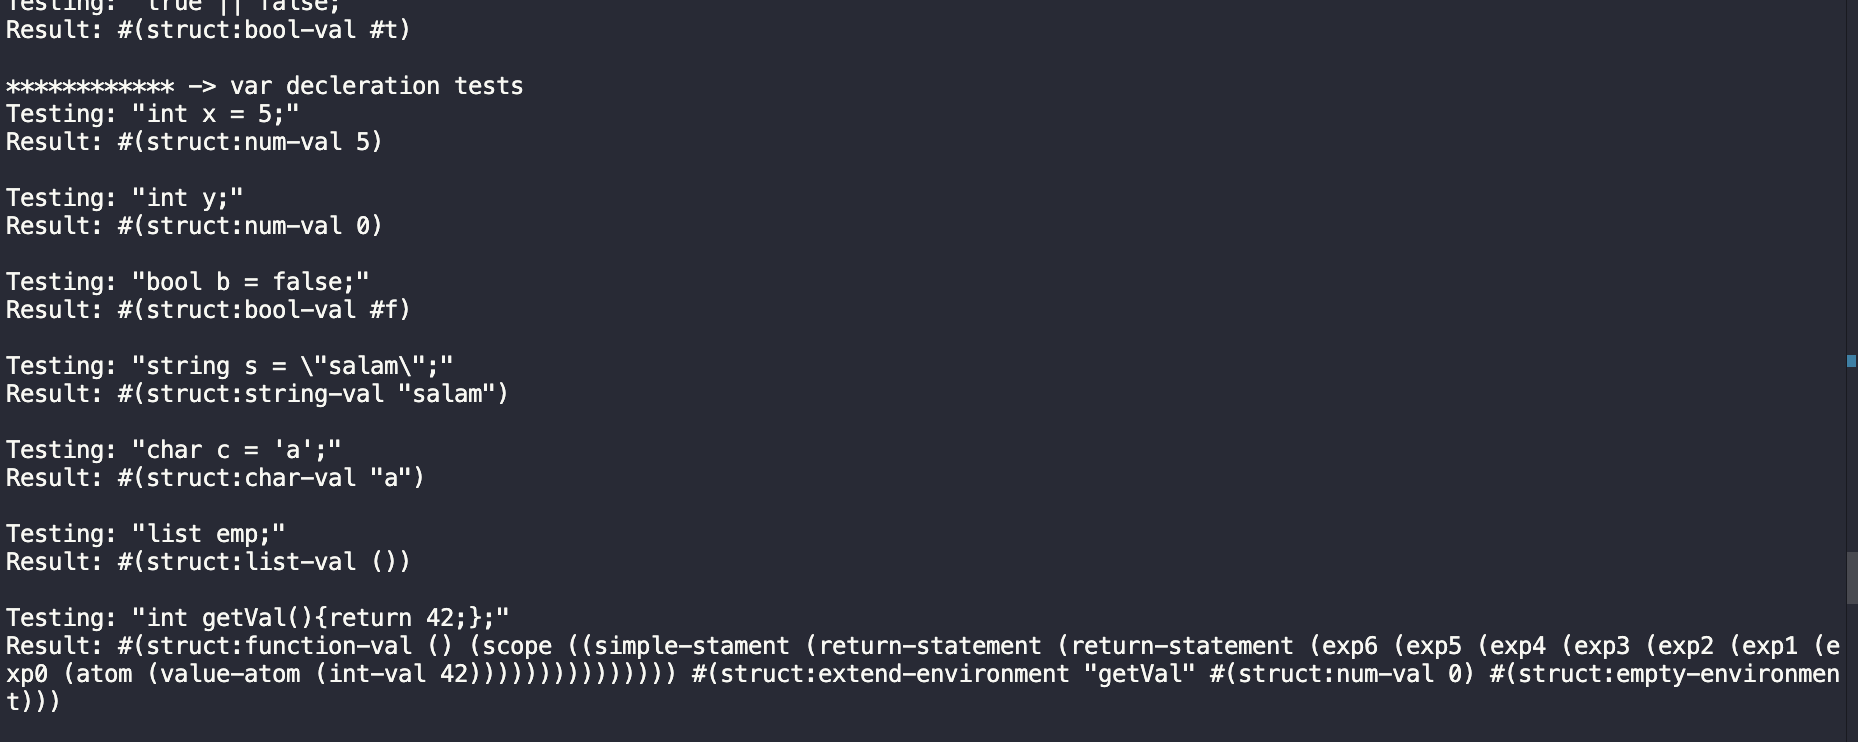
\includegraphics[width=1\linewidth]{pics/var1.png}
        \caption{بخشی از تست‌بنچ ساده، همچنین لازم به ذکر است مقدار دهی اولیه به لیست در زبان برای‌ ساده‌سازی ممکن نیست و باید با push های متوالی اینکار انجام شود.}
\end{figure}
\subsection{\lr{function handling}}
توابع مانند روش کتاب، به چشم یک متغیر دیده می‌شوند، همچنین با استفاده از روشی مانند روش کتاب برای پیاده‌سازی 
\lr{letrec}
امکان تعریف تابع بازگشتی نیز وجود دارد.
\begin{figure}[h]
        \centering
        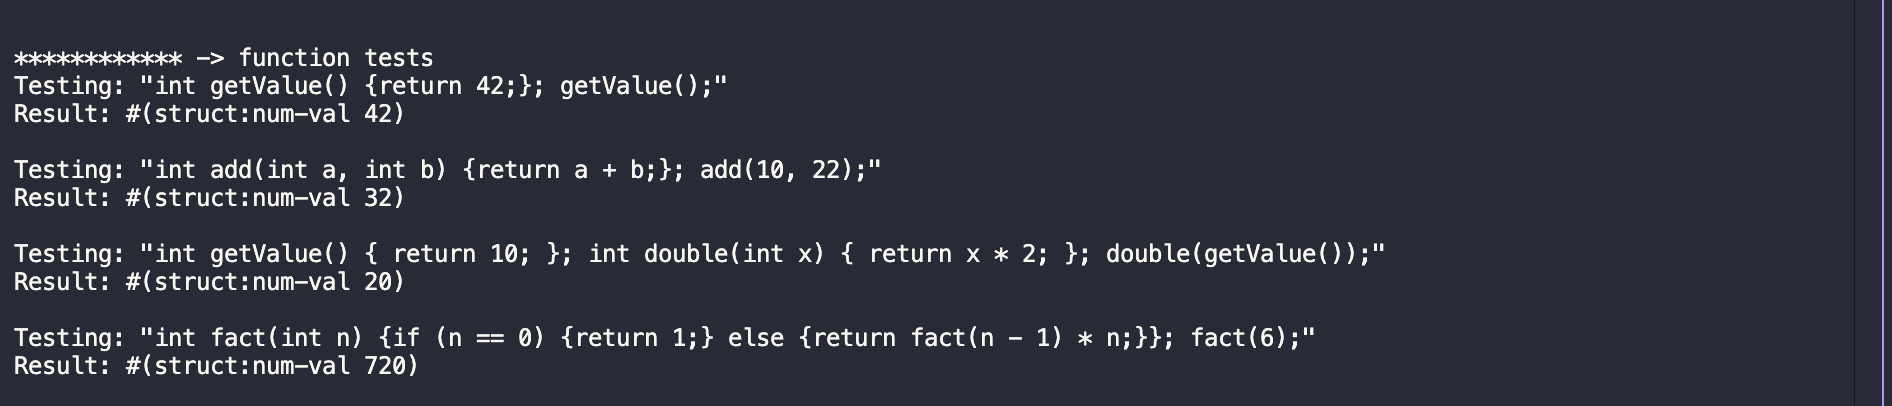
\includegraphics[width=1\linewidth]{pics/func1.png}
        \caption{بخشی از تست‌های ساده برای توابع}
\end{figure}
\subsection{\lr{Lazy Evalutation}}
دقیقا استراکچر‌‌هایی مانند 
\lr{thunk}
در زبان پیاده‌سازی نشده، اما سعی شده اگر می‌شد، در محاسبه 
\lr{value-of}
هر نود 
\lr{AST}
اگر بچه سمت چپ کافی بود، بچه سمت راست را حساب نکنیم(تنها در آپریشن‌هایی که شبیه سی، به صورت لیزی ایولیویت می‌شوند، طبعا این روش کارایی شبیه \lr{thunk} را ندارد اما اندکی به بهبود زمان اجرا کمک می‌کند.)
\subsection{\lr{Memory Management}}
همه منابع داخل اسکوپ تعریف شده و خارج اسکوپ غیر قابل دسترسی هستند.
\section{ارزیابی عبارات}
TODO
\section{مدیریت خطا}
برای مدیریت خطا، از کتاب‌خانه 
\lr{eopl}
استفاده شده، همچنین به علت تایپ استریکت بودن زبان پیاده‌سازی شده، مدیریت‌ خطا‌ها کمی آسان‌تر از حالت عادی‌ است.
\\
برای مدیریت خطا، جز ۲ مورد(یکی در برای گرفتن مقدار وریبلی که در انوایرمنت نیست و دیگری و دیگری برای کستینگ ناموفق در دیتاتایپ‌ها)
همه خطا‌ها مربوط به اکسپرشن ایولیویشن هستند، و به راحتی حین ایولیوت کردن، قابل پیشبینی هستند، برای مثال وقتی 
\lr{valud-of}
برای اکسپرشن از نوع تقسیم پیاده‌سازی می‌شود، کافیست تا اگر ولیو‌آف سمت راست ۰ بود، توسط 
\lr{eopl::error}
خطای دیویژن بای زیرو داده شود.
\\
هنگام بروز خطا نوع خطا و همچنین پیام مرتبط با آن نمایش‌داده می‌شود و اجرای برنامه متوقف می‌شود، نتایج تست بنچ ارور هندلینگ در زیر آمده که نشان می‌دهد 
همه خطا‌هایی که در داک ذکر شده بود برسی شده‌اند، همچنین، خطا‌های بیشتری فرای آنچه در داک گفته شده، پیاده‌سازی شده‌اند.
\\
\begin{figure}[h]
        \centering
        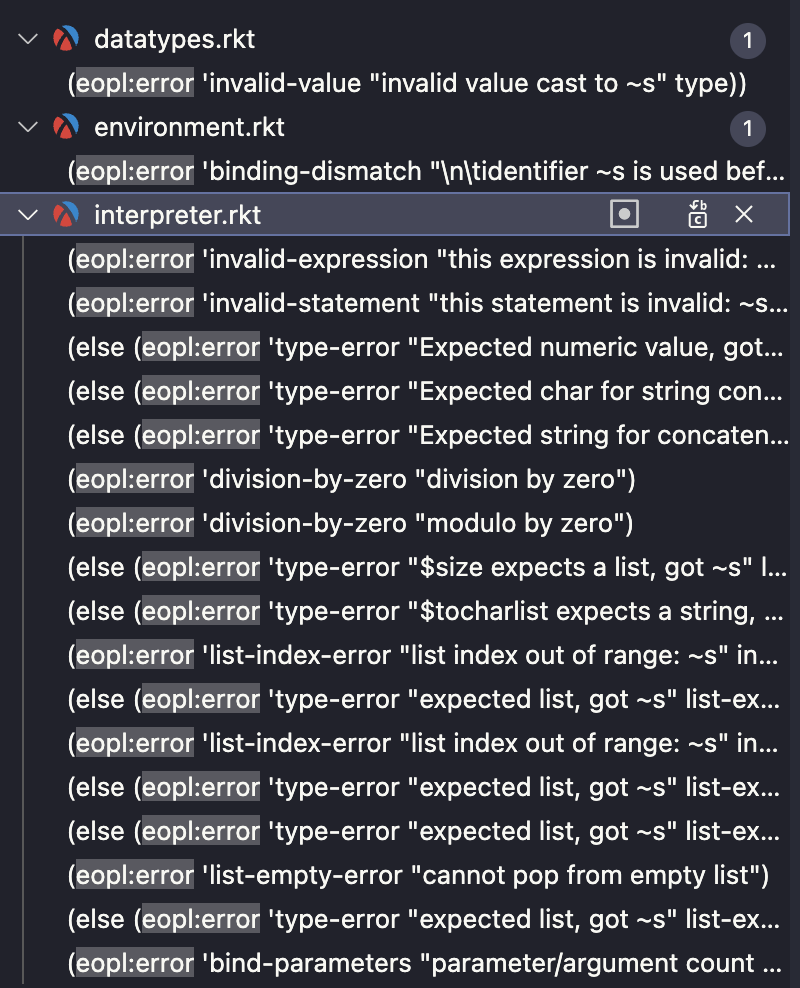
\includegraphics[width=0.5\linewidth]{pics/eopl.png}
        \caption{تمام‌ خطا‌هایی که در زبان از آنها ساپورت می‌شود}
\end{figure}

\begin{figure}[h]
           \centering
        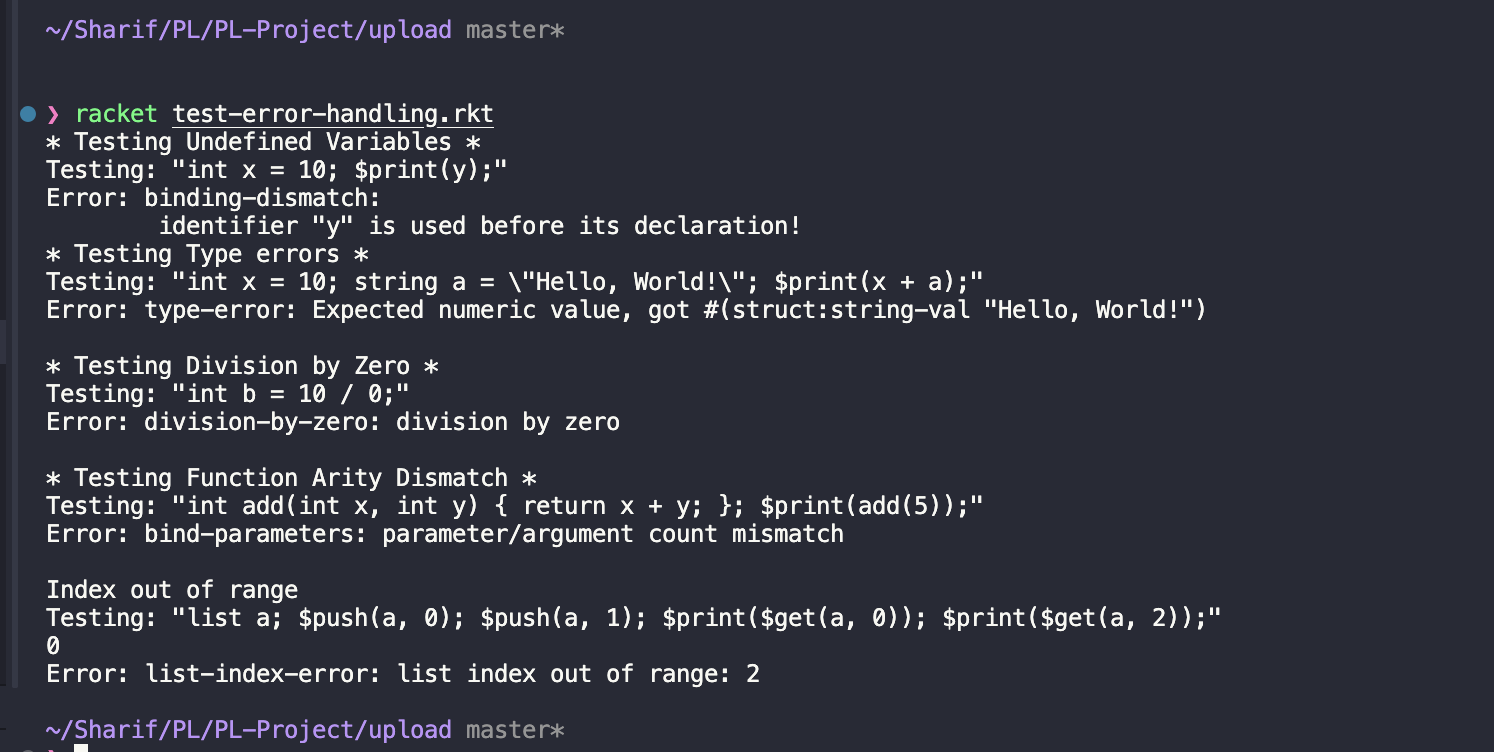
\includegraphics[width=1\linewidth]{pics/error-tb.png}
        \caption{نتیجه تست بنچ ارور هندلینگ، دقت کنید اجرای هر برنامه در این تست بنچ در یک ترای‌کچ قرار دارد تا در صورت بروز خطا، برنامه متوقف نشود و همه تست‌ها اجرا شوند.}     
\end{figure}
\FloatBarrier
\section{TypeChecker}
TODO
\section{نتایج تست‌بنچ ها}

\end{document}


